\header{
    \section{La Belle et le Cantonnier} \label{la-belle-et-le-cantonnier}
    %
    %chanson datant du début du 19eme siècle
    %
    \insertComment{Sur l'air de "Sur la route de Louviers".}{Chantée par Colette Renard début XXème.}
}

\enluminure{4}{\href{https://www.youtube.com/watch?v=WYW6JeMGFhE}{S}}{ur} la route de Louviers \bissimple 
\\Il y avait un cantonnier\bissimple 
\\Et qui baisait \bissimple 
\\Et qui baisait comme un voyou  
\\Au lieu d'casser des cailloux  
\\\\Une belle dame vient à passer \bissimple 
\\Dans un beau carosse doré \bissimple 
\\Elle y baisait \bissimple 
\\Elle y baisait comne un voyou  
\\A en fair' craquer les roues  
\\\\Elle aperçut le cantonnier \bissimple 
\\Dans le fond d'un grand fossé \bissimple 
\\Et qui baisait \bissimple 
\\Et qui baisait comme un voyou  
\\Une fillette aux cheveux roux  
\\\\Elle lui dit: "Brave cantonnier \bissimple 
\\Avec moi veux-tu monter ? \bissimple 
\\Pour me baiser \bissimple 
\\Pour me baiser comme un voyou
\\Le préfet est mon époux"  
\\\\A ces mots, le cantonnier \bissimple 
\\Laisse la rousse dans le fossé \bissimple 
\\Et va baiser \bissimple 
\\Et va baiser comme un voyou  
\\La belle dame pleine de bijoux  
\bisdouble{Le lendemain par arrêté }
{Fut nommé chef cantonnier}
\\Parce qu'il baisait \bissimple 
\\Parce qu'il baisait comme un voyou  
\\Au lieu de casser des cailloux  
\\\\Voici la moralité \bissimple
\\Dans la vie pour arriver \bissimple
\\Il faut baiser \bissimple
\\Il faut baiser comm' des voyous  
\\Les bell's dam's qui ont des sous! \bissimple
\\
\bigskip
\begin{figure}[h!]
\centering
   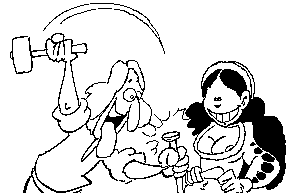
\includegraphics[width=1\textwidth]{images/cantonnier.png}
 \end{figure}
\breakpage